% LAB 11: Web Scraping
%
% CSE/IT 107: Introduction to Programming
% New Mexico Tech
%
% Prepared by Russell White and Christopher Koch and Tyler Cecil
% Fall 2014
\documentclass[11pt]{cselabheader}
\usepackage{multicol,graphicx}

%%%%%%%%%%%%%%%%%% SET TITLES %%%%%%%%%%%%%%%%%%%%%%%%%
\fancyhead[R]{Lab 11: Web Scraping}
\title{Lab 11: Web Scraping}

\begin{document}

\maketitle

\hrule
\begin{quotation}
``The limits of my language mean the limits of my world.''
\end{quotation}
\begin{flushright}
--- Ludwig Wittgenstein
\end{flushright}

\begin{quotation}
``Any sufficiently advanced technology is indistinguishable from magic.''
\end{quotation}
\begin{flushright}
--- Arthur Clarke
\end{flushright}

\begin{quotation}
``Imagination is more important than knowledge.''
\end{quotation}
\begin{flushright}
--- Albert Einstein
\end{flushright}

\hrule

\section{Introduction}

In this lab, you will be extracting information from web pages and learning how
to plot some of it.

You may be familiar with the Wikipedia game of clicking on the first link and
figuring out how long it takes you to arrive at the Philosophy page. You will be
writing a Python script that starts at a Wikipedia page and does this to figure
out how many clicks it takes.

\pagebreak

\section{HTML}

As you may be familiar, HTML is the main formatting language of the
Internet. HTML stands for HyperText Markup Language. As a language, it
defines where content appears on a website, and how it looks. For an
example, open up \texttt{Google Chrome} and navigate to
\texttt{http://www.nmt.edu}. Right click on the webpage, and select
``View Source''. What follows is the source code for \texttt{nmt.edu}!

HTML is actually fairly easy to read. All content exists between
various kinds of ``tags''. Each tag has a special kind of
meaning. Here is a simple example:

\begin{lstlisting}[style=python, language=html]
<!DOCTYPE html>
<html>
  <head>
    <title>Hello!</title>
  </head>
  <body>
    <p> This is a paragraph in the body of the page </p>
    <p> This text is <b> BOLD </b></p>
  </body>
</html>
\end{lstlisting}

The tags \lstinline!html!, \lstinline!head!, and \lstinline!body! are required
for a web page and just give some structure. \lstinline!head! contains
information about the page, such as the title. \lstinline!body! contains the
actual content of the web page. The special \lstinline{<!DOCTYPE html>} also has
to be there.

To learn about all the various tags, see
\begin{center}
\url{http://www.w3schools.com/}.
\end{center}

\section{Requesting a web page}

The following is an example code snippet to get the source code of a particular
web page:
\begin{lstlisting}
from urllib import request

def get_page_source(webpage):
  req = request.Request(webpage, headers={'User-Agent' : 'Python Browser'})
  page = request.urlopen(req)
  return page.read()

print(get_page_source('https://cs.nmt.edu/~ckoch/cse107/beautifulsoup.html'))
\end{lstlisting}

This will give you the HTML source of the web address you give it.

Below is an example of a slightly more complex program using urllib. This
program gets a random Wikipedia article and prints out its URL. This
is identical to what would happen if you click on the Random Article button
on the Wikipedia homepage.

\lstinputlisting[style=python]{lab11/random_wikipage.py}

All of the logic for this program is inside the \lstinline{get_random}
function. First, it creates a \lstinline{Request} object. This is used
to tell urllib what page we want to load. First, we construct our URL using
the \lstinline{base} variable (since all of our URLs are going to start the
same way), then we pass a special headers argument. Don't worry too much about
what headers are -- in this case, we are only specifying a \lstinline{User-Agent}
string in order to identify ourselves to the remote server. We need to do this
because the default urllib \lstinline{User-Agent} string is blocked by
Wikipedia.

Once we have our \lstinline{Request} object created, we simply pass it to
\lstinline{request.urlopen} in order to get an object representing the page
we've loaded. Creating the \lstinline{Request} object and calling
\lstinline{request.urlopen} will be done no matter what page we are loading.

Once we have the page object, we simply check its URL (since the Wikipedia
random article button redirects you to a new page, this will not be the
same URL that we requested!) and strip off the beginning section, leaving
us with only /wiki/Article.

\pagebreak
\section{BeautifulSoup}
BeautifulSoup is a library that will let you ``scrape'' web pages for certain
information. Instead of having to deal with the HTML source of a web page
directly, you can use BeautifulSoup to find information easily.
If, for example, I want to find all the \texttt{a} elements (link
elements) on a web page, I could do the following:

\begin{lstlisting}[caption={BeautifulSoup},label={lst:bs}]
import bs4

# Using previous function
data = get_page_source('https://cs.nmt.edu/~ckoch/cse107/beautifulsoup.html')
soup = bs4.BeautifulSoup(data)

print(soup.prettify())

elements = soup.findAll('a')
print(elements)
\end{lstlisting}

The output of \lstinline!.prettify()! looks like this:
\begin{lstlisting}[language=HTML]
<!DOCTYPE html>
<html>
 <head>
  <title>
   CSE107 BeautifulSoup Test
  </title>
 </head>
 <body>
  <p>
   Haha
  </p>
  <p>
   <a href="https://cs.nmt.edu/~ckoch/">
    Chris's site
   </a>
   <a href="https://arctem.com">
    Russell's site
   </a>
  </p>
 </body>
</html>
\end{lstlisting}

On this page, we have two \texttt{a} elements, and thus
\lstinline!.findAll()! returns the following list:
\begin{lstlisting}[style=bash]
[<a href="https://cs.nmt.edu/~ckoch/">Chris's site</a>,
<a href="https://arctem.com">Russell's site</a>]
\end{lstlisting}

Now, to find just the first element, we use the \lstinline!.find()! function.
Also note that the above list is not a list of strings; the type of the list
elements is a beautiful soup element tag. These tags have a few properties, as
you can see in the following example:

\begin{lstlisting}[caption={BeautifulSoup tag usage},label={lst:tag}]
import bs4
# calling beautiful soup with my own data
soup = bs4.BeautifulSoup('<html><body><p>Test</p><p>T</p></body></html>')

paragraph = soup.find('p') # finds <p>Test</p>
print(paragraph)
print(paragraph.string) # Test
print(paragraph.contents) # ['Test']
print(paragraph.name) # prints p

body = soup.find('body') # finds <body><p>Test</p></body>
print(body.contents) # [<p>Test</p>, <p>T</p>]
print(body.string) # None, because there is more than one thing
\end{lstlisting}

\subsection{Summary}

Tables~\ref{tab:bsmeth} and~\ref{tab:bsatt} show the BeautifulSoup methods and
the tag attributes we will probably need in this lab. If you want to know more
about BeautifulSoup, take a look at its documentation:
\begin{center}
  \url{http://www.crummy.com/software/BeautifulSoup/bs4/doc/}
\end{center}

\begin{table}[!ht]
  \centering
  \begin{tabular}{p{3cm} p{11cm}}
    \toprule
    \bfseries Method & \bfseries What it does \\
    \midrule
    \lstinline!s.find(name)! & Finds the first tag named \lstinline!name! in
    document \lstinline!s! \\
    \lstinline!s.findAll(name)! & Finds all tags named \lstinline!name! in
    document \lstinline!s! \\
    \lstinline!s.prettify()! & Returns a string of the HTML formatted prettily
    \\
    \bottomrule
  \end{tabular}
  \caption{BeautifulSoup methods, where \lstinline!s! is a BeautifulSoup object.
    See Listings~\ref{lst:bs} and~\ref{lst:tag} for example usage.}
  \label{tab:bsmeth}
\end{table}

\begin{table}[!ht]
  \centering
  \begin{tabular}{p{2cm} p{12cm}}
    \toprule
    \bfseries Attribute & \bfseries What it gives \\
    \midrule
    \lstinline!.contents! & List of all the things a tag contains \\
    \lstinline!.name! & Name of the tag (e.g. \texttt{p} or \texttt{title}) \\
    \lstinline!.string! & If \lstinline!.contents! only contains one thing,
    return a string of that. Otherwise, \lstinline!None! since it will not know
    which one to choose \\
    \bottomrule
  \end{tabular}
  \caption{Tag attributes. See Listing~\ref{lst:tag} for example usage.}
  \label{tab:bsatt}
\end{table}


\pagebreak
\section{Matplotlib}

Matplotlib is a neat library for plotting in Python. It works similarly to
MATLAB plotting so that people with experience in that can easily switch over;
however, we will give you our own introduction to it.

Let's plot the following $x$ and $y$ coordinates:

\begin{table}[!ht]
  \centering
  \begin{tabular}{ llllllllllll }
    \bfseries x & 0 & 2 & 4 & 6 & 8 & 10 & 12 & 14 & 16 & 18\\
    \midrule
    \bfseries y & 0 & 4 & 8 & 12 & 16 & 20 & 24 & 28 & 32 & 36
  \end{tabular}
  \caption{Values for Figure~\ref{fig:x-2x}}
  \label{tab:x-2x}
\end{table}

\begin{lstlisting}[caption={Code to produce Figure~\ref{fig:x-2x}} with values from Table~\ref{tab:x-2x},label={lst:x-2x}]
import matplotlib.pylab as pl

x = range(0, 20, 2)
y = range(0, 40, 4)
pl.plot(x, y, '.')
pl.xlabel('X values')
pl.ylabel('Y values')
pl.title('Random plot of X vs Y')
pl.show()
\end{lstlisting}

\begin{figure}[!ht]
  \centering
  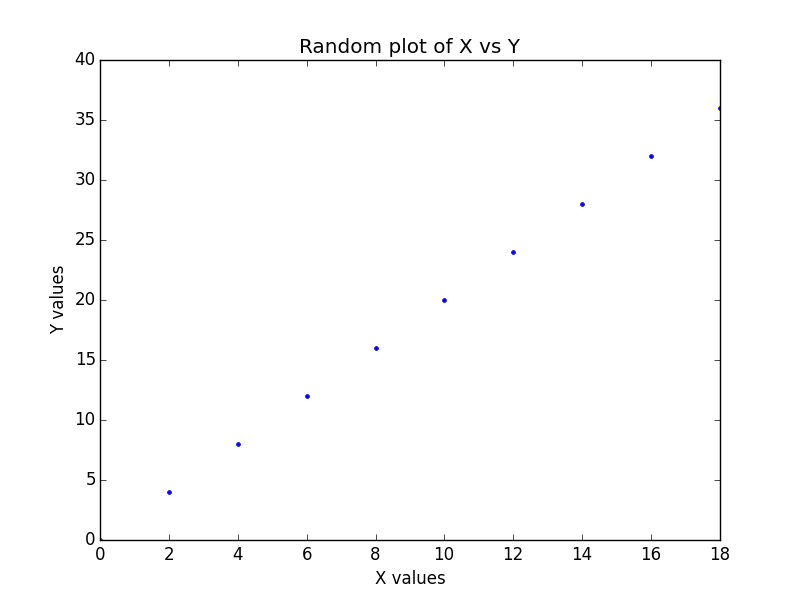
\includegraphics[width=0.8\textwidth]{lab11/x-2x-plot.png}
  \caption{Graph produced by Listing~\ref{lst:x-2x}}
  \label{fig:x-2x}
\end{figure}

The \lstinline!pl.plot()! function takes as arguments a sequence for x, a
sequence for y, and optionally a formatting specifier. The important ones are
``-'' for a solid line and ``.'' for point markers. You can add more options,
such as colors or labels. You can find more docs on
these specifiers on the Matploblib website:
\begin{center}
  \url{http://matplotlib.org/api/pyplot_api.html#matplotlib.pyplot.plot}
\end{center}

You have to call \lstinline!pl.show()! for the graph to actually show. There are
ways to print the graphs to image files, but we are not covering those for now.
You can look them up in the documentation if you want.

Bar plots work in a similar way. The \lstinline!pl.bar()! takes a sequence of
numbers to label the left side of the bars with and a sequence of heights of the
bars.

\begin{lstlisting}[caption={Code to produce Figure~\ref{fig:x-2x-bar}},label={lst:x-2x-bar}]
import matplotlib.pylab as pl

x = range(1, 11, 2)
y = range(1, 21, 4)
pl.bar(x, y)
pl.show()
\end{lstlisting}

\begin{figure}[!ht]
  \centering
  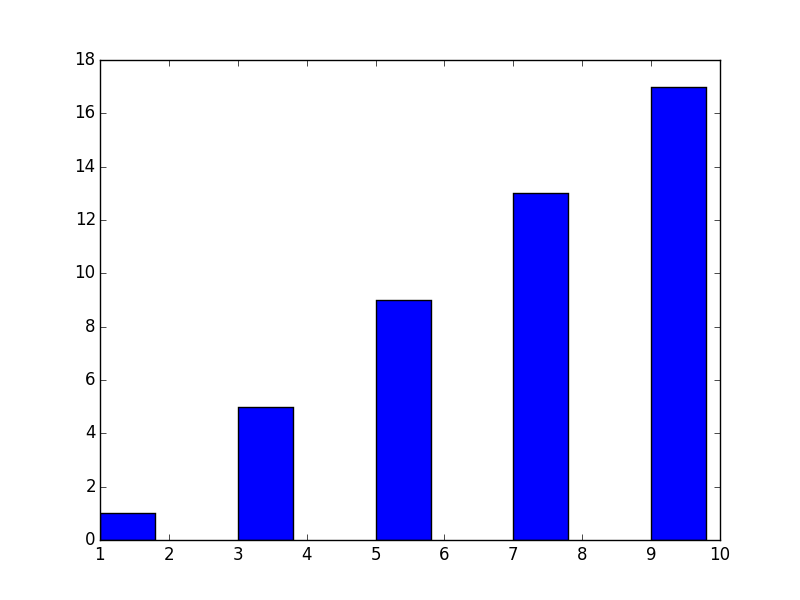
\includegraphics[width=0.8\textwidth]{lab11/x-2x-bar-plot.png}
  \caption{Graph produced by Listing~\ref{lst:x-2x-bar}}
  \label{fig:x-2x-bar}
\end{figure}

These are the two main functions you will need for plotting in this lab. If you
want to customize more, please see the matplotlib pylab documentation at
\begin{center}
  \url{http://matplotlib.org/api/pyplot_summary.html}.
\end{center}

\pagebreak

\section{Exercises}
\label{sec:ex}

%One exerscis for soup (like get the title of a page)
%One for matplotlib (plot x^2)
%The main project

\begin{warningbox}{Boilerplate}
  Remember that this lab \emph{must} use the
  boilerplate syntax introduced in Lab~5.
\end{warningbox}

\begin{description}
  \item[simple\_plot.py] Using Matplotlib, make a simple plot of the function
    $y = x^2$ to make sure that you are able to use matplotlib.

  \item[beautiful\_title.py] Like the last exercise, just to make sure the
    libraries are working properly, use \texttt{get\_page\_source} and
    \texttt{BeautifulSoup} to get the title of a user-entered Wikipedia page.

  \item[wiki\_stats.py] This comprises the majority of the project. Your task
    takes advantage of the ``philosophy property'' of most Wikipedia pages. The
    user will provide a list of Wikipedia article names. Your program will take
    this list, and return a list of the ``first-link-distance'' to Philosophy.
    That is, the number of articles you must visit in order to reach Philosophy,
    (\url{https://en.wikipedia.org/wiki/Philosophy})
    if for each article you simply follow the first link in the main body of the
    article (that is, ignoring the italicized text for the article, such as
    ``for other uses...'' or ``did you mean...'') that is not in the pronunciation
    guide (in which case most articles would lead to Latin) and does not lead to
    a Wikipedia Help or Meta page.
        
    If the given article does not converge to Philosophy, display the string
    ``inft''.  It the given article does not exist, display the string ``N/A''.

    \emph{Take a look at the provided wikiclicker.py for a function that gets
      you the first link on a Wikipedia page, automatically applying the above
      rules}

    For example, see this sample input and output (the numbers here are just
    made up, don't worry):
    \begin{lstlisting}[style=bash]
Article List: NASA, Space, Grapefruit, BadArticle
Philosophy Distance: [16, 8, inft, N/A]
    \end{lstlisting}
    So this means that three clicks from ``NASA'', you can find ``Philosophy'',
    but ``Grapefruit'' never reaches ``Philosophy''. ``Bad Article'' is not
    found.

    If the user list was empty, however, generate a random list of 5 articles.
    For example:
    \begin{lstlisting}[style=bash]
Article List:
Choosing random articles...
Articles: Dog, Cat, Roger Ebert, Star Wars, Philosophy
Philosophy Distance: [9, 11, 18, 20, 6]
    \end{lstlisting}

    Finally, your program must \textbf{plot a bar graph} of the distance of each
    article, with labeled axes, identifying each bar. If the distance was
    ``N/A'' or ``inft'', then do not plot that article.

    \begin{center}
      \url{http://en.wikipedia.org/wiki/Wikipedia:Getting_to_Philosophy}
    \end{center}

\end{description}

\pagebreak
\section{Submitting}

Files to submit:
\begin{itemize}
\item simple\_plot.py (Section~\ref{sec:ex})
\item beautiful\_title.py (Section~\ref{sec:ex})
\item wiki\_stats.py (Section~\ref{sec:ex})
\end{itemize}

You may submit your code as either a tarball (instructions below) or as a .zip
file. Either one should contain all files used in the exercises for this lab.
The submitted file should be named either
\texttt{cse107\_firstname\_lastname\_lab11.zip} or
\texttt{cse107\_firstname\_lastname\_lab11.tar.gz} depending on which method you
used.

For Windows, use a tool you like to create a \texttt{.zip} file. The TCC
computers should have \texttt{7z} installed. For Linux, look at lab 1 for
instructions on how to create a tarball or use the ``Archive Manager'' graphical
tool.

\begin{center}
  \textbf{Upload your tarball or .zip file to Canvas.}
\end{center}

\end{document}
